\section{System Overview}
\label{sec:system_overview}

This section presents the architecture of our multi-agent code generation system, describing the logical pipeline, difficulty estimation mechanism, escalation policy, and the experimental configurations evaluated in this study.

% -----------------------------------------------------------------------------
\subsection{Multi-Agent Pipeline Architecture}
\label{subsec:pipeline}

The proposed multi-agent pipeline decomposes the code generation task into five specialized components, each responsible for a distinct phase of the development process. The pipeline follows the sequence: \textbf{Planner} $\rightarrow$ \textbf{Router} $\rightarrow$ \textbf{Developer} $\rightarrow$ \textbf{Tester} $\rightarrow$ \textbf{Reviewer}, with conditional looping upon test failure.

The \textbf{Planner} agent receives the task specification and estimates its difficulty using Scrum-style story points, providing a rationale for the assessment. The \textbf{Router} uses this difficulty estimate to select an appropriately-sized Developer model, balancing computational cost against task complexity. The \textbf{Developer} agent generates the implementation code based on the task description and, in retry iterations, incorporates feedback from previous failures. The \textbf{Tester} is a non-LLM component that executes the generated code against assertion-based tests in a sandboxed environment. Finally, the \textbf{Reviewer} agent analyzes the test results and provides actionable feedback for subsequent iterations without modifying the code directly.

Figure~\ref{fig:architecture_overview} illustrates the four architectural configurations evaluated in this study, highlighting the differences in pipeline structure and model allocation.

\begin{figure}[ht]
    \centering
    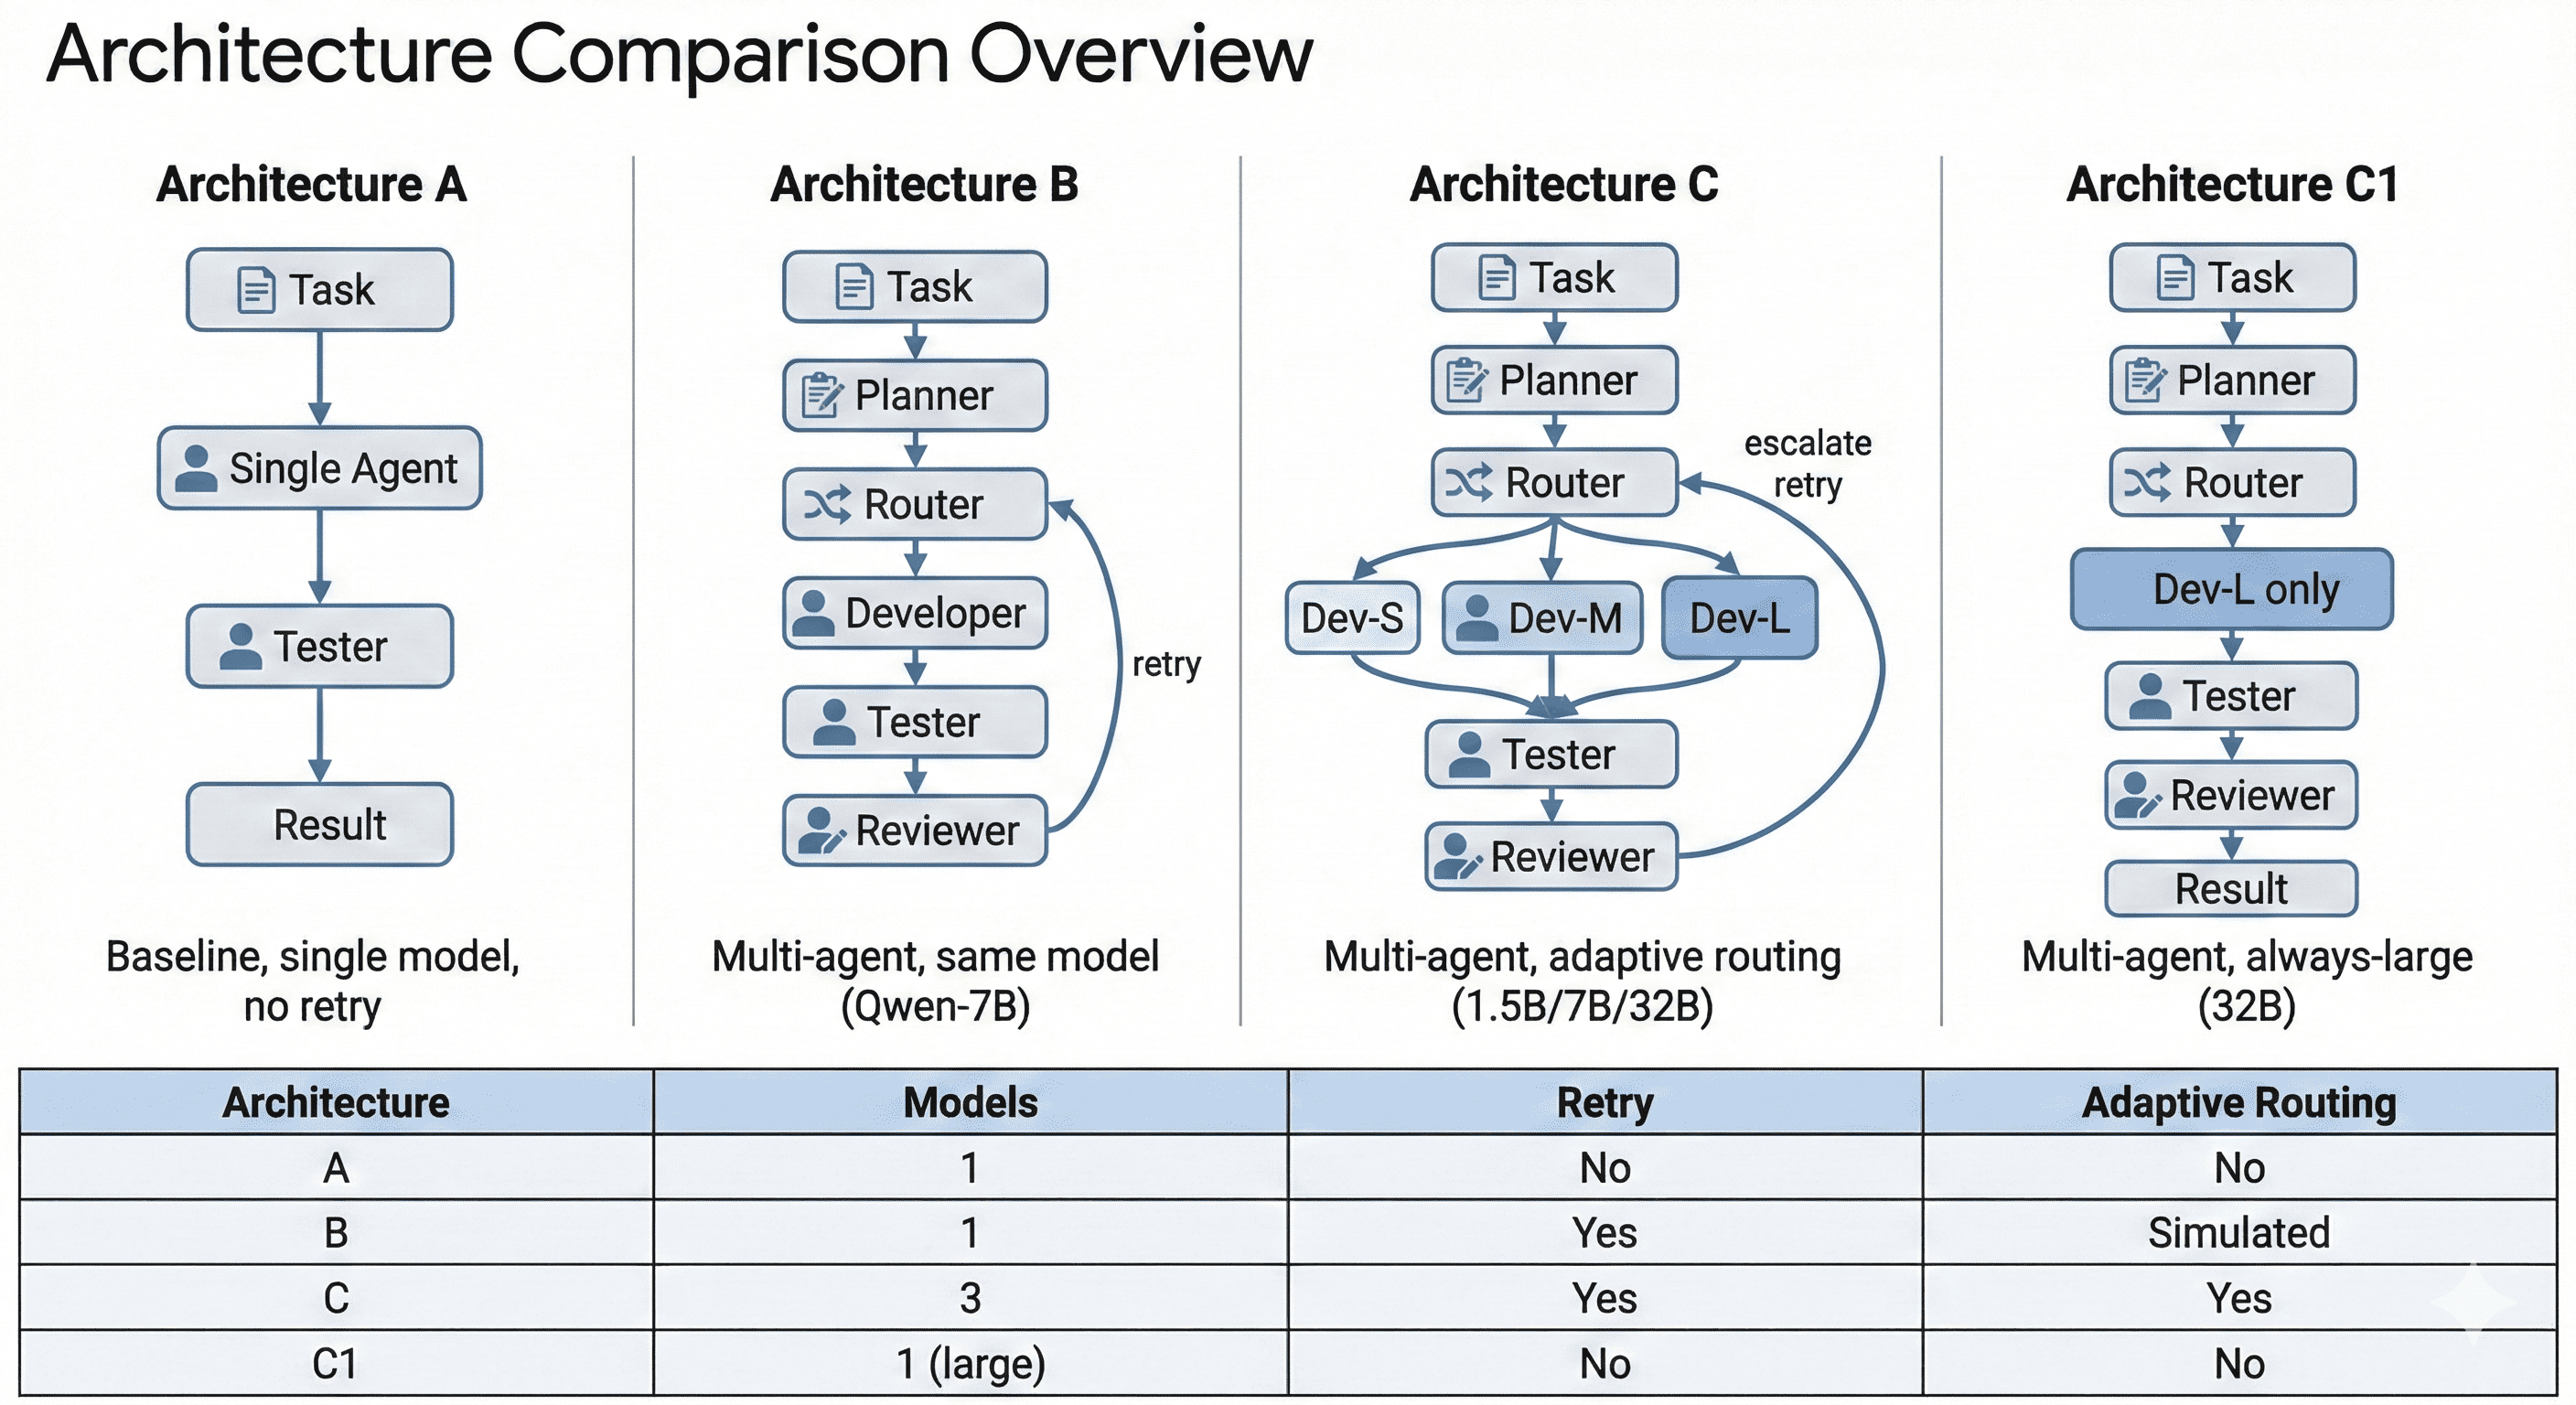
\includegraphics[width=\columnwidth]{figures/ArchitetureOverview.png}
    \caption{Comparison of the four experimental architectures: (A) single-agent baseline, (B) multi-agent with single model, (C) multi-agent with adaptive routing across three model tiers, and (C1) multi-agent always using the largest model.}
    \label{fig:architecture_overview}
\end{figure}

% -----------------------------------------------------------------------------
\subsection{Difficulty Estimation via Story Points}
\label{subsec:story_points}

Task difficulty estimation is performed by the Planner agent using a Fibonacci-based story point scale: \{1, 2, 3, 5, 8\}. This scale, borrowed from Agile software development practices, serves as a routing signal rather than a time estimate. The Planner evaluates each task along five dimensions: (1) algorithmic complexity, (2) edge case density, (3) external constraints such as performance requirements or strict I/O formatting, (4) coupling with other components, and (5) specification ambiguity.

Story points are mapped to developer tiers as follows: points 1--2 indicate trivial to small tasks routed to the smallest model (Tier S), points 3--5 represent medium to challenging tasks routed to a mid-sized model (Tier M), and point 8 denotes hard tasks requiring the largest model (Tier L). This mapping is visualized in Figure~\ref{fig:story_points_routing}.

\begin{figure}[ht]
    \centering
    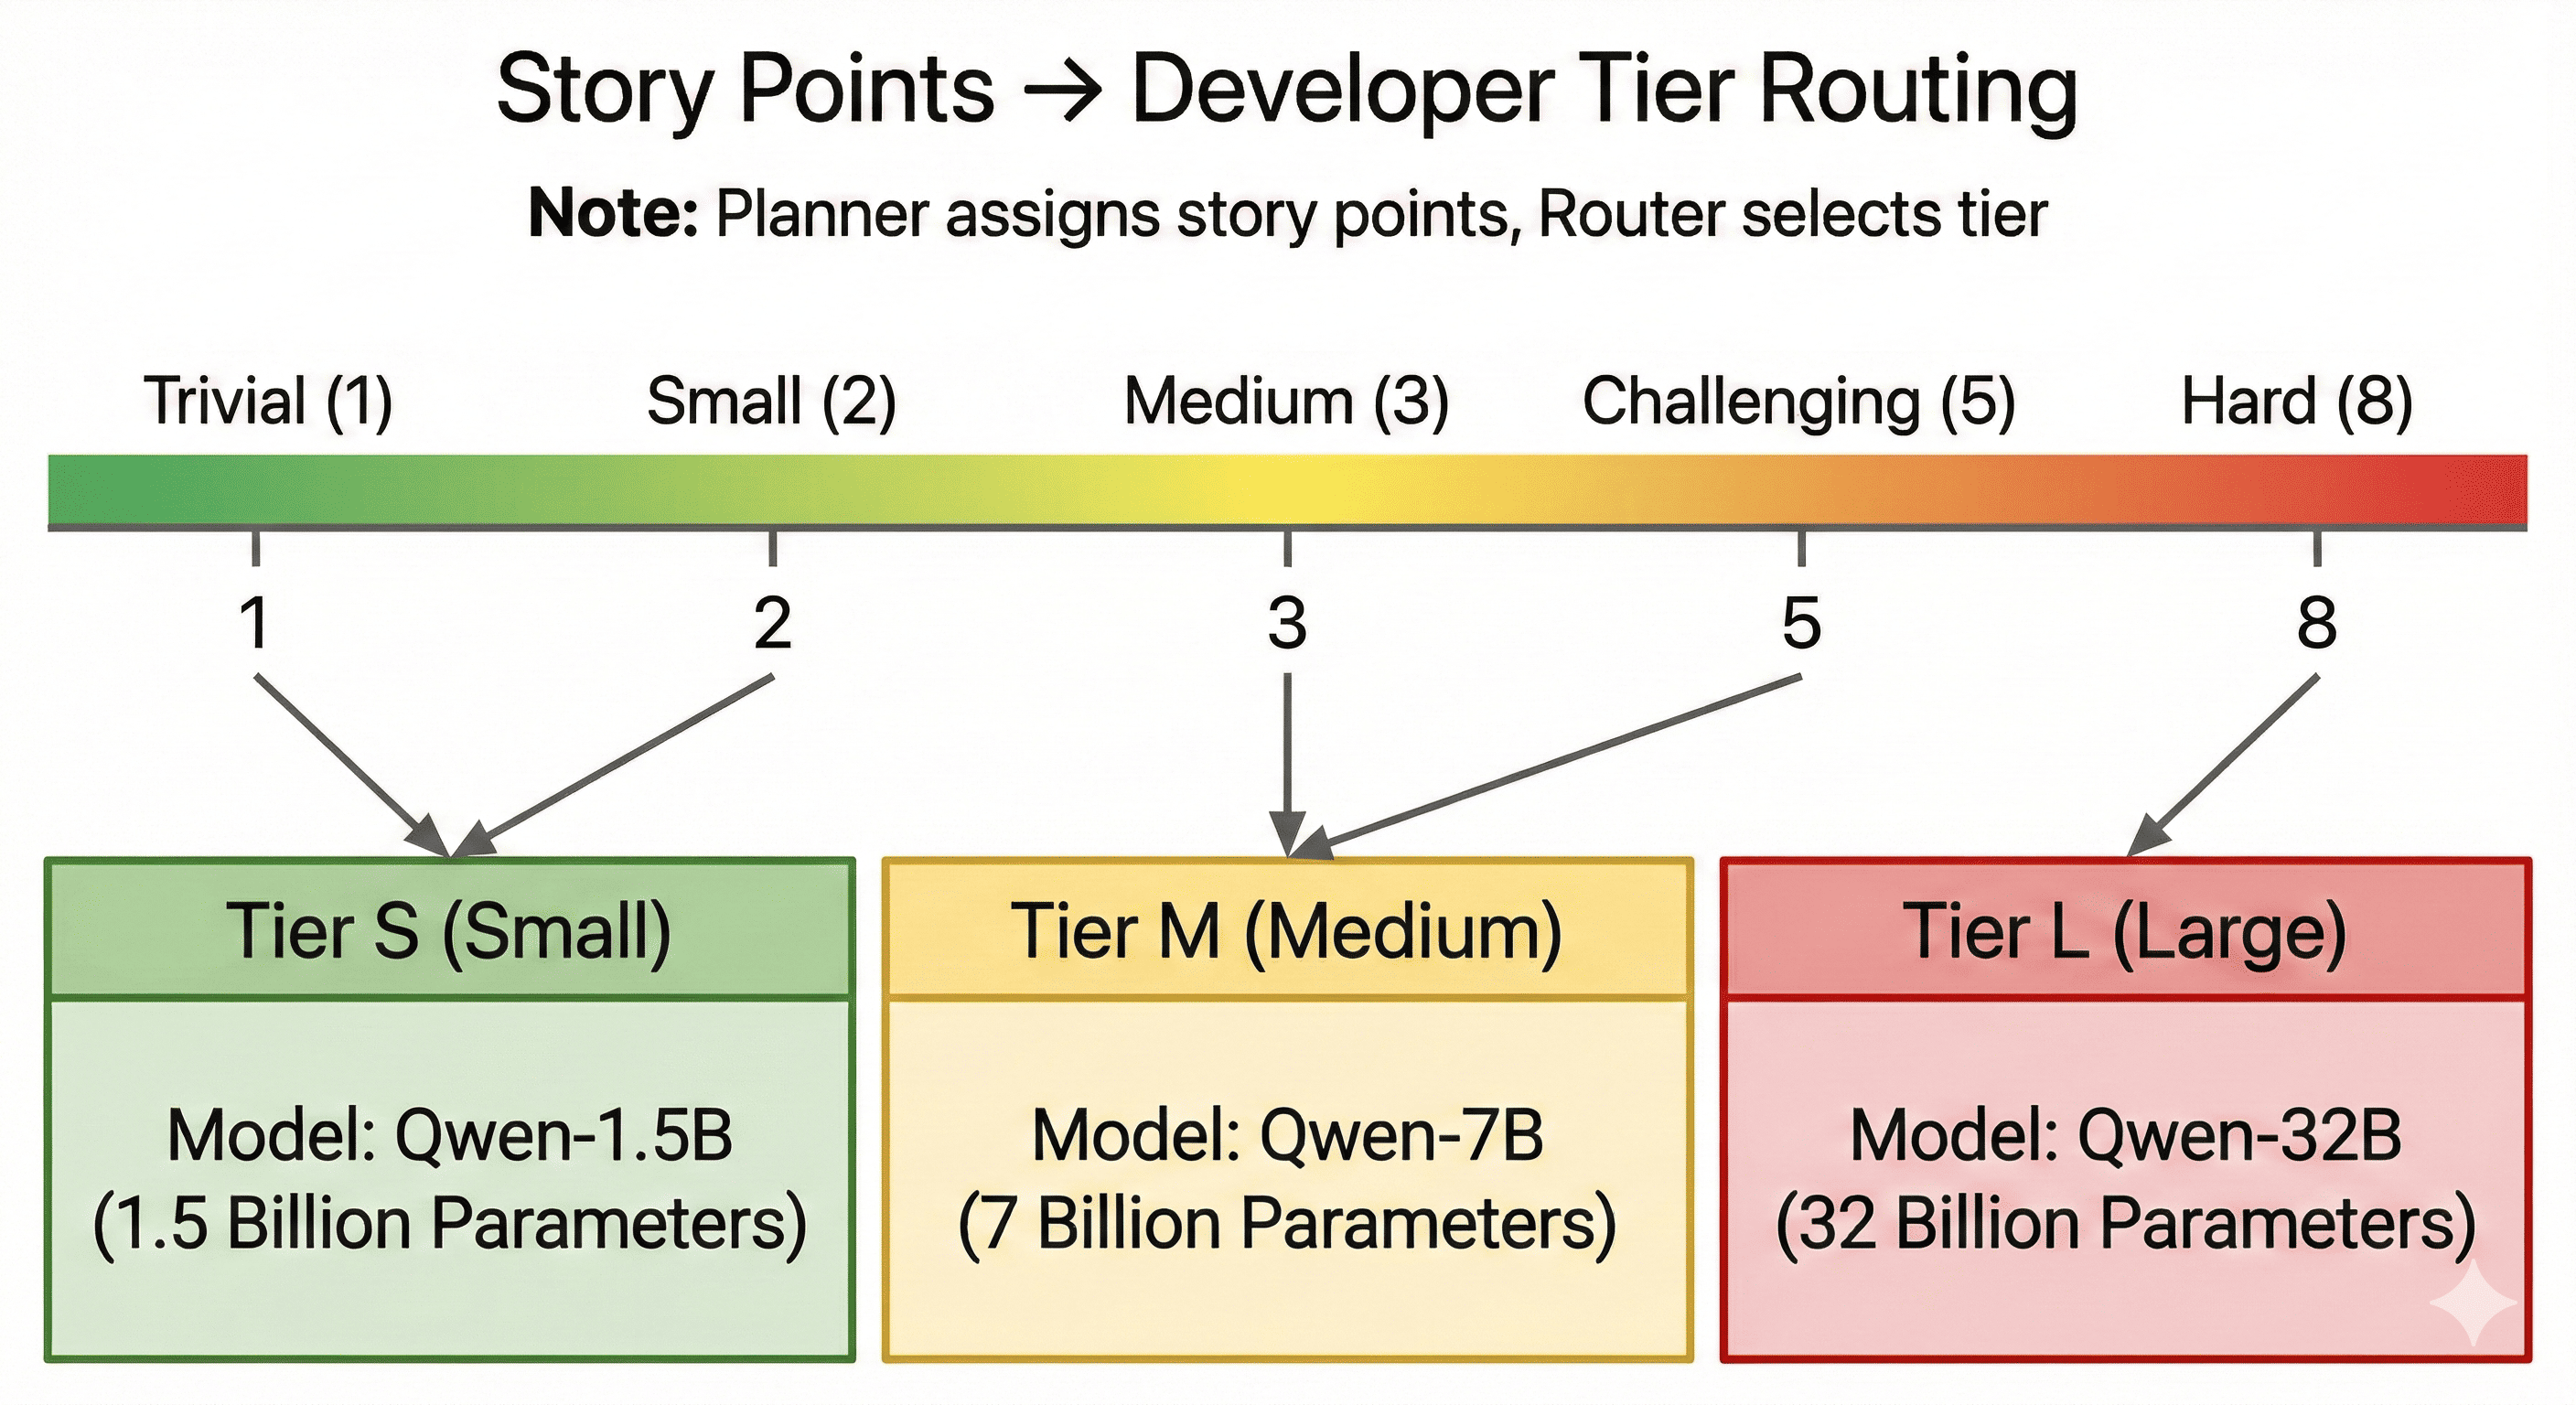
\includegraphics[width=\columnwidth]{figures/StoryPointsTierRouting.png}
    \caption{Mapping from story points to developer tiers. Each tier corresponds to a different model capacity: Tier S (1.5B parameters), Tier M (7B parameters), and Tier L (32B parameters).}
    \label{fig:story_points_routing}
\end{figure}

% -----------------------------------------------------------------------------
\subsection{Adaptive Routing and Escalation Policy}
\label{subsec:escalation}

The system implements an adaptive escalation policy that progressively increases model capacity upon test failure. When the Tester reports a failure, the Router escalates the task to the next tier: S $\rightarrow$ M $\rightarrow$ L. A maximum of two escalations is permitted, after which the pipeline terminates regardless of test outcome.

Upon escalation, the Developer receives the previous code, failure history (error messages from test execution), and feedback from the Reviewer. This accumulated context enables the stronger model to address specific deficiencies identified in prior attempts. Figure~\ref{fig:escalation_policy} illustrates the escalation flow and termination conditions.

\begin{figure}[ht]
    \centering
    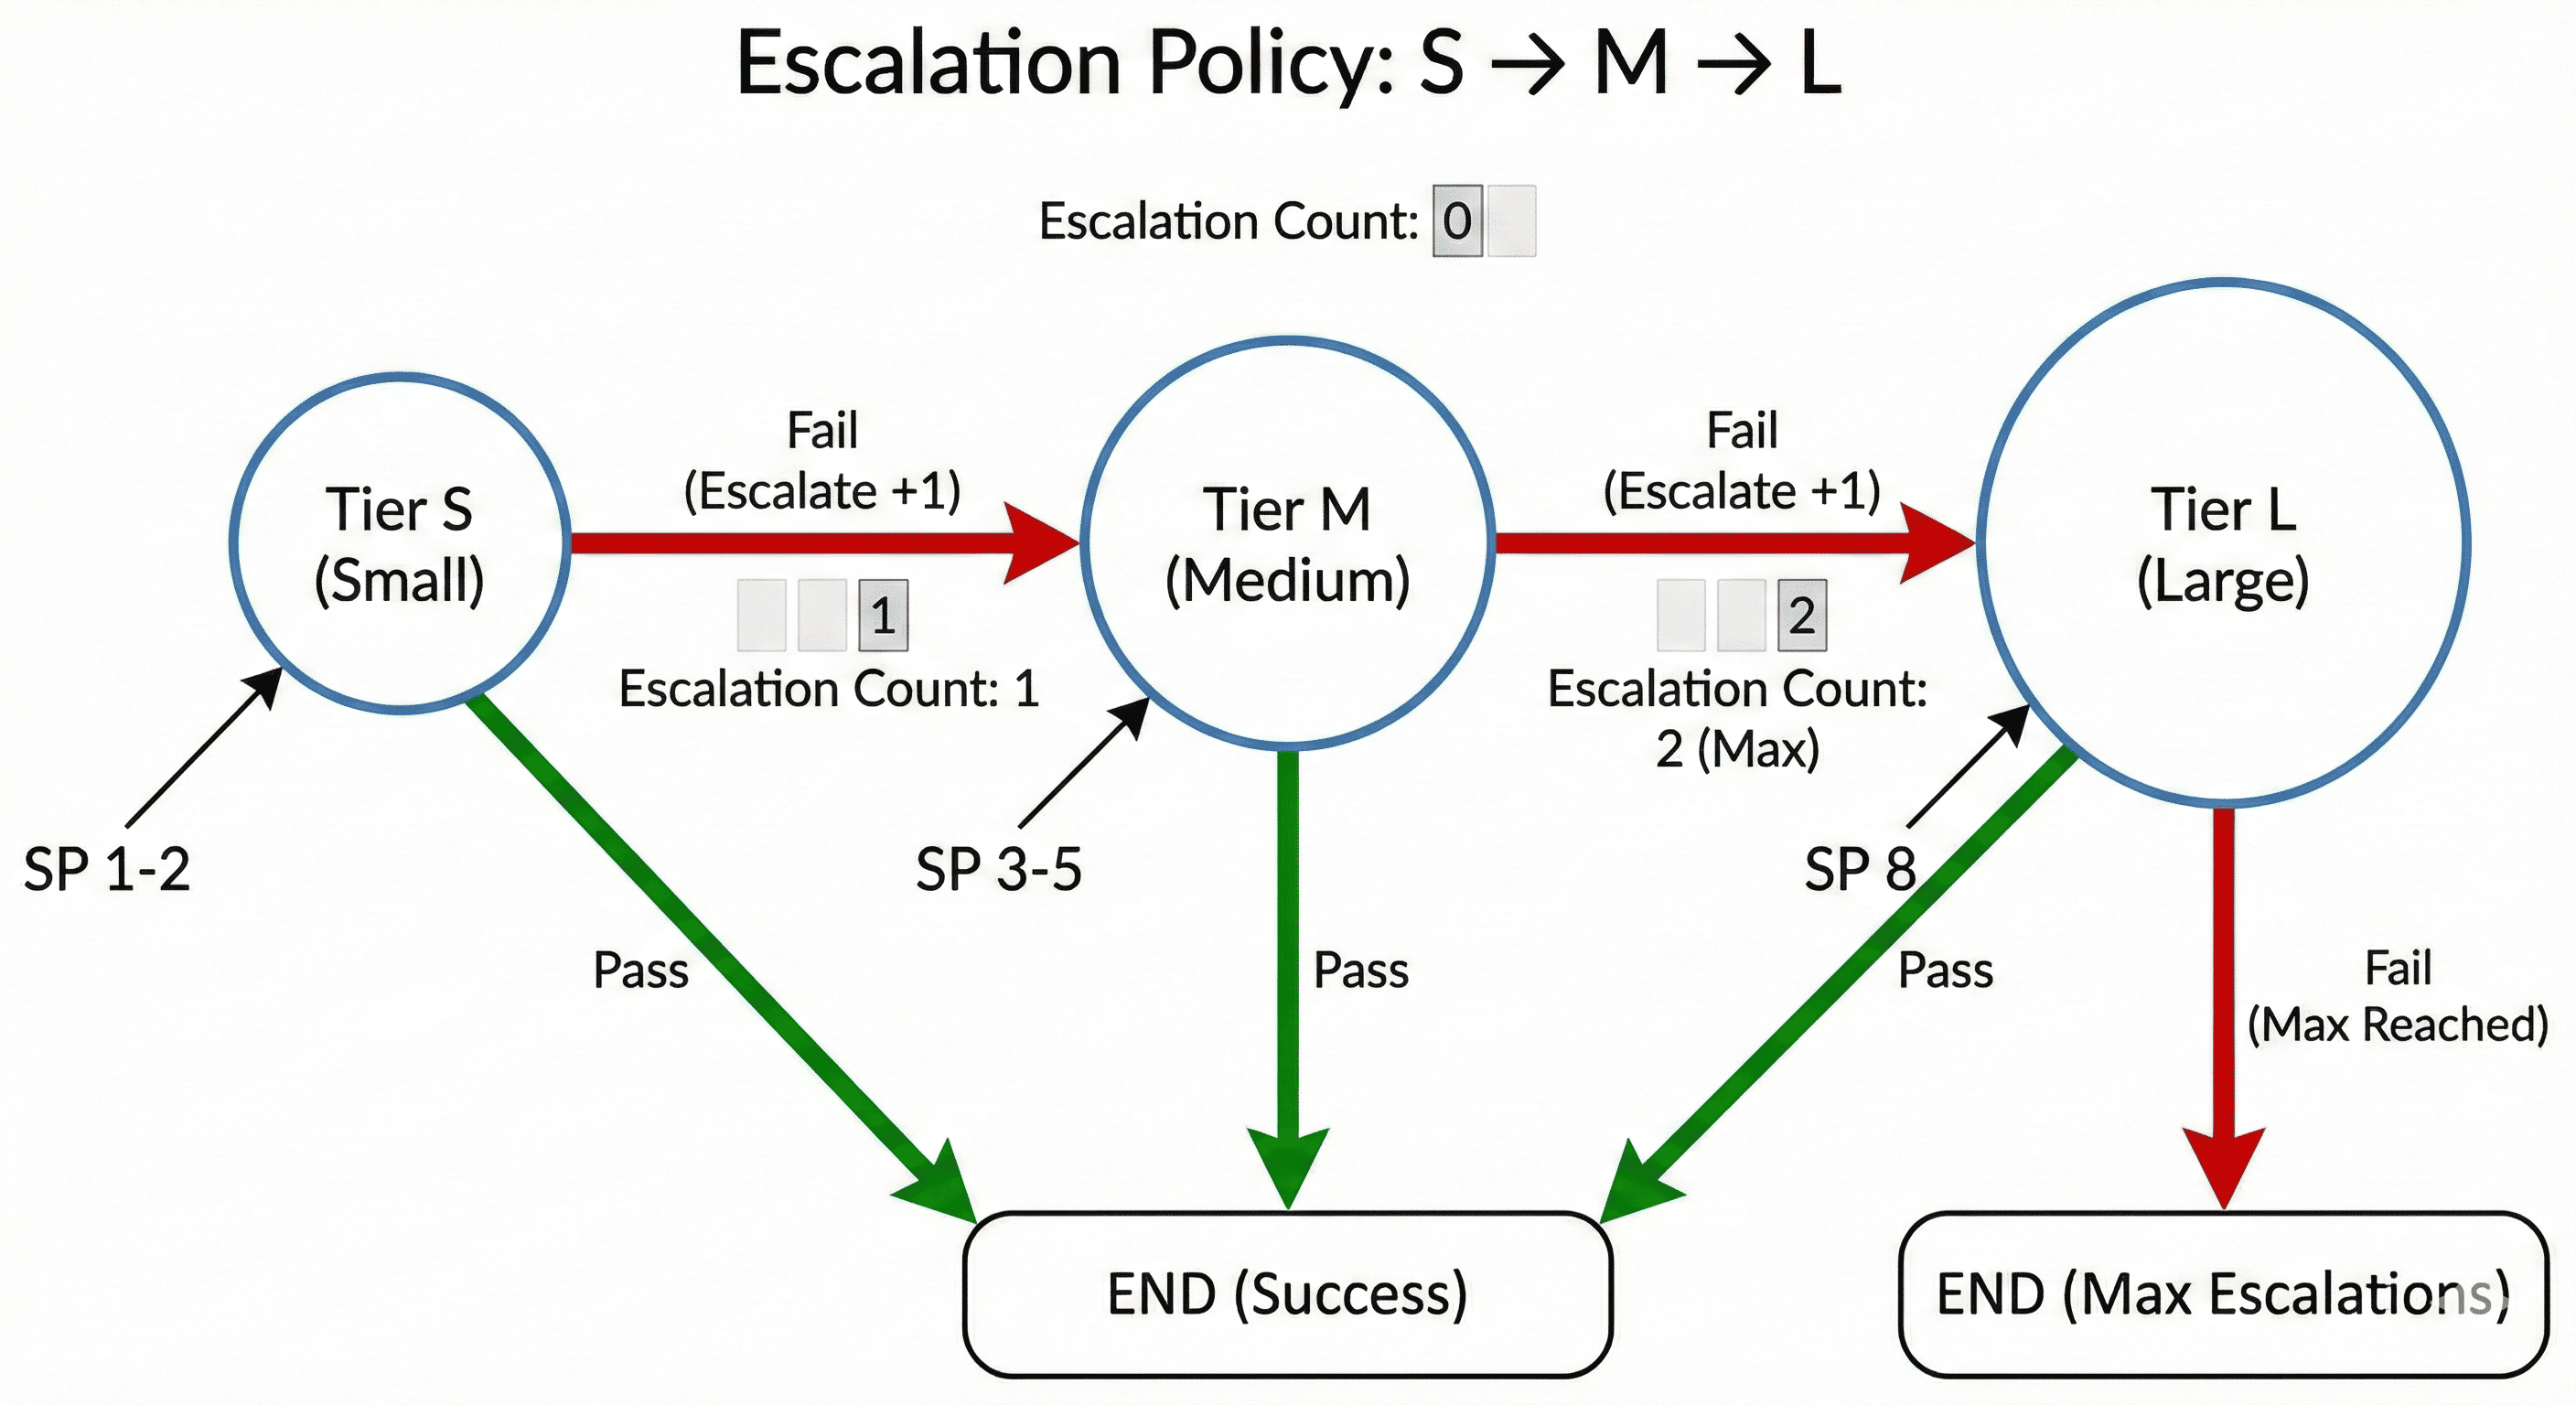
\includegraphics[width=\columnwidth]{figures/EscalationPolicy.png}
    \caption{Escalation policy flow. On test failure, the system escalates from Tier S to M to L. The pipeline terminates upon test success or after reaching maximum escalations.}
    \label{fig:escalation_policy}
\end{figure}

% -----------------------------------------------------------------------------
\subsection{Experimental Architectures}
\label{subsec:architectures}

We evaluate five architectural configurations to isolate the effects of multi-agent orchestration, model specialization, and adaptive routing:

\textbf{Architecture A} serves as the single-agent baseline. A single LLM receives the task and generates code in one pass without planning, review, or retry mechanisms.

\textbf{Architecture B} introduces the full multi-agent pipeline while keeping the model constant. All roles (Planner, Developer (all tiers), and Reviewer) use the same model. This configuration isolates the effect of role separation and iterative refinement from model capacity differences.

\textbf{Architecture C} employs specialized models for each role. The Planner and Reviewer use a generalist model suited for reasoning and analysis. The Developer role uses capacity-matched models: a small model (1.5B) for Tier S, a medium model (7B) for Tier M, and a large model (32B) for Tier L.

\textbf{Architecture C1} is a variant of C that bypasses adaptive routing by always using the Tier L developer (32B model), regardless of the Planner's difficulty estimate. This configuration serves as an upper-bound reference for comparing the efficiency-quality trade-off of adaptive routing.

\textbf{Architecture C2} is an ablation study that removes the Tier S developer entirely. Tasks that would normally route to Tier S are instead handled by Tier M from the start. This configuration tests whether the smallest model tier is beneficial or introduces unnecessary failure cascades.

Table~\ref{tab:model_config} summarizes the model assignments for each architecture.

\begin{table}[ht]
    \centering
    \footnotesize
    \setlength{\tabcolsep}{4pt}
    \begin{tabular}{l|ccccc}
        \toprule
        \textbf{Role} & \textbf{A} & \textbf{B} & \textbf{C} & \textbf{C1} & \textbf{C2} \\
        \midrule
        Planner  & ---  & Q-7B  & L-8B   & L-8B   & L-8B \\
        Dev-S    & ---  & Q-7B  & Q-1.5B & ---    & --- \\
        Dev-M    & ---  & Q-7B  & Q-7B   & ---    & Q-7B \\
        Dev-L    & ---  & Q-7B  & Q-32B  & Q-32B  & Q-32B \\
        Reviewer & ---  & Q-7B  & L-8B   & L-8B   & L-8B \\
        Baseline & Q-7B & ---   & ---    & ---    & --- \\
        \bottomrule
    \end{tabular}
    \caption{Model assignments per architecture. Q = Qwen2.5-Coder-Instruct, L = Meta-Llama-3-Instruct. Numbers indicate model size in billions of parameters.}
    \label{tab:model_config}
\end{table}

% -----------------------------------------------------------------------------
\subsection{Prompt Repetition Technique}
\label{subsec:prompt_repetition}

We investigate the effect of prompt repetition, a technique recently proposed by Leviathan et al.~\cite{leviathan2025prompt} for improving non-reasoning LLM performance. The technique transforms the user prompt from $\langle$\textsc{query}$\rangle$ to $\langle$\textsc{query}$\rangle$\texttt{\textbackslash n\textbackslash n}$\langle$\textsc{query}$\rangle$, duplicating the input with a newline separator.

The rationale is that LLMs are causal language models where each token can only attend to preceding tokens. By repeating the prompt, tokens in the second occurrence can attend to all tokens in the first occurrence, potentially improving comprehension of complex instructions. The overhead is approximately 2$\times$ input tokens during the prefill stage, with no change to output token count. Figure~\ref{fig:prompt_repetition} visualizes this attention pattern difference.

For each base architecture (A, B, C), we evaluate a corresponding prompt repetition variant (A-PR, B-PR, C-PR), applying repetition to all user-facing prompts while leaving system prompts unchanged.

\begin{figure}[ht]
    \centering
    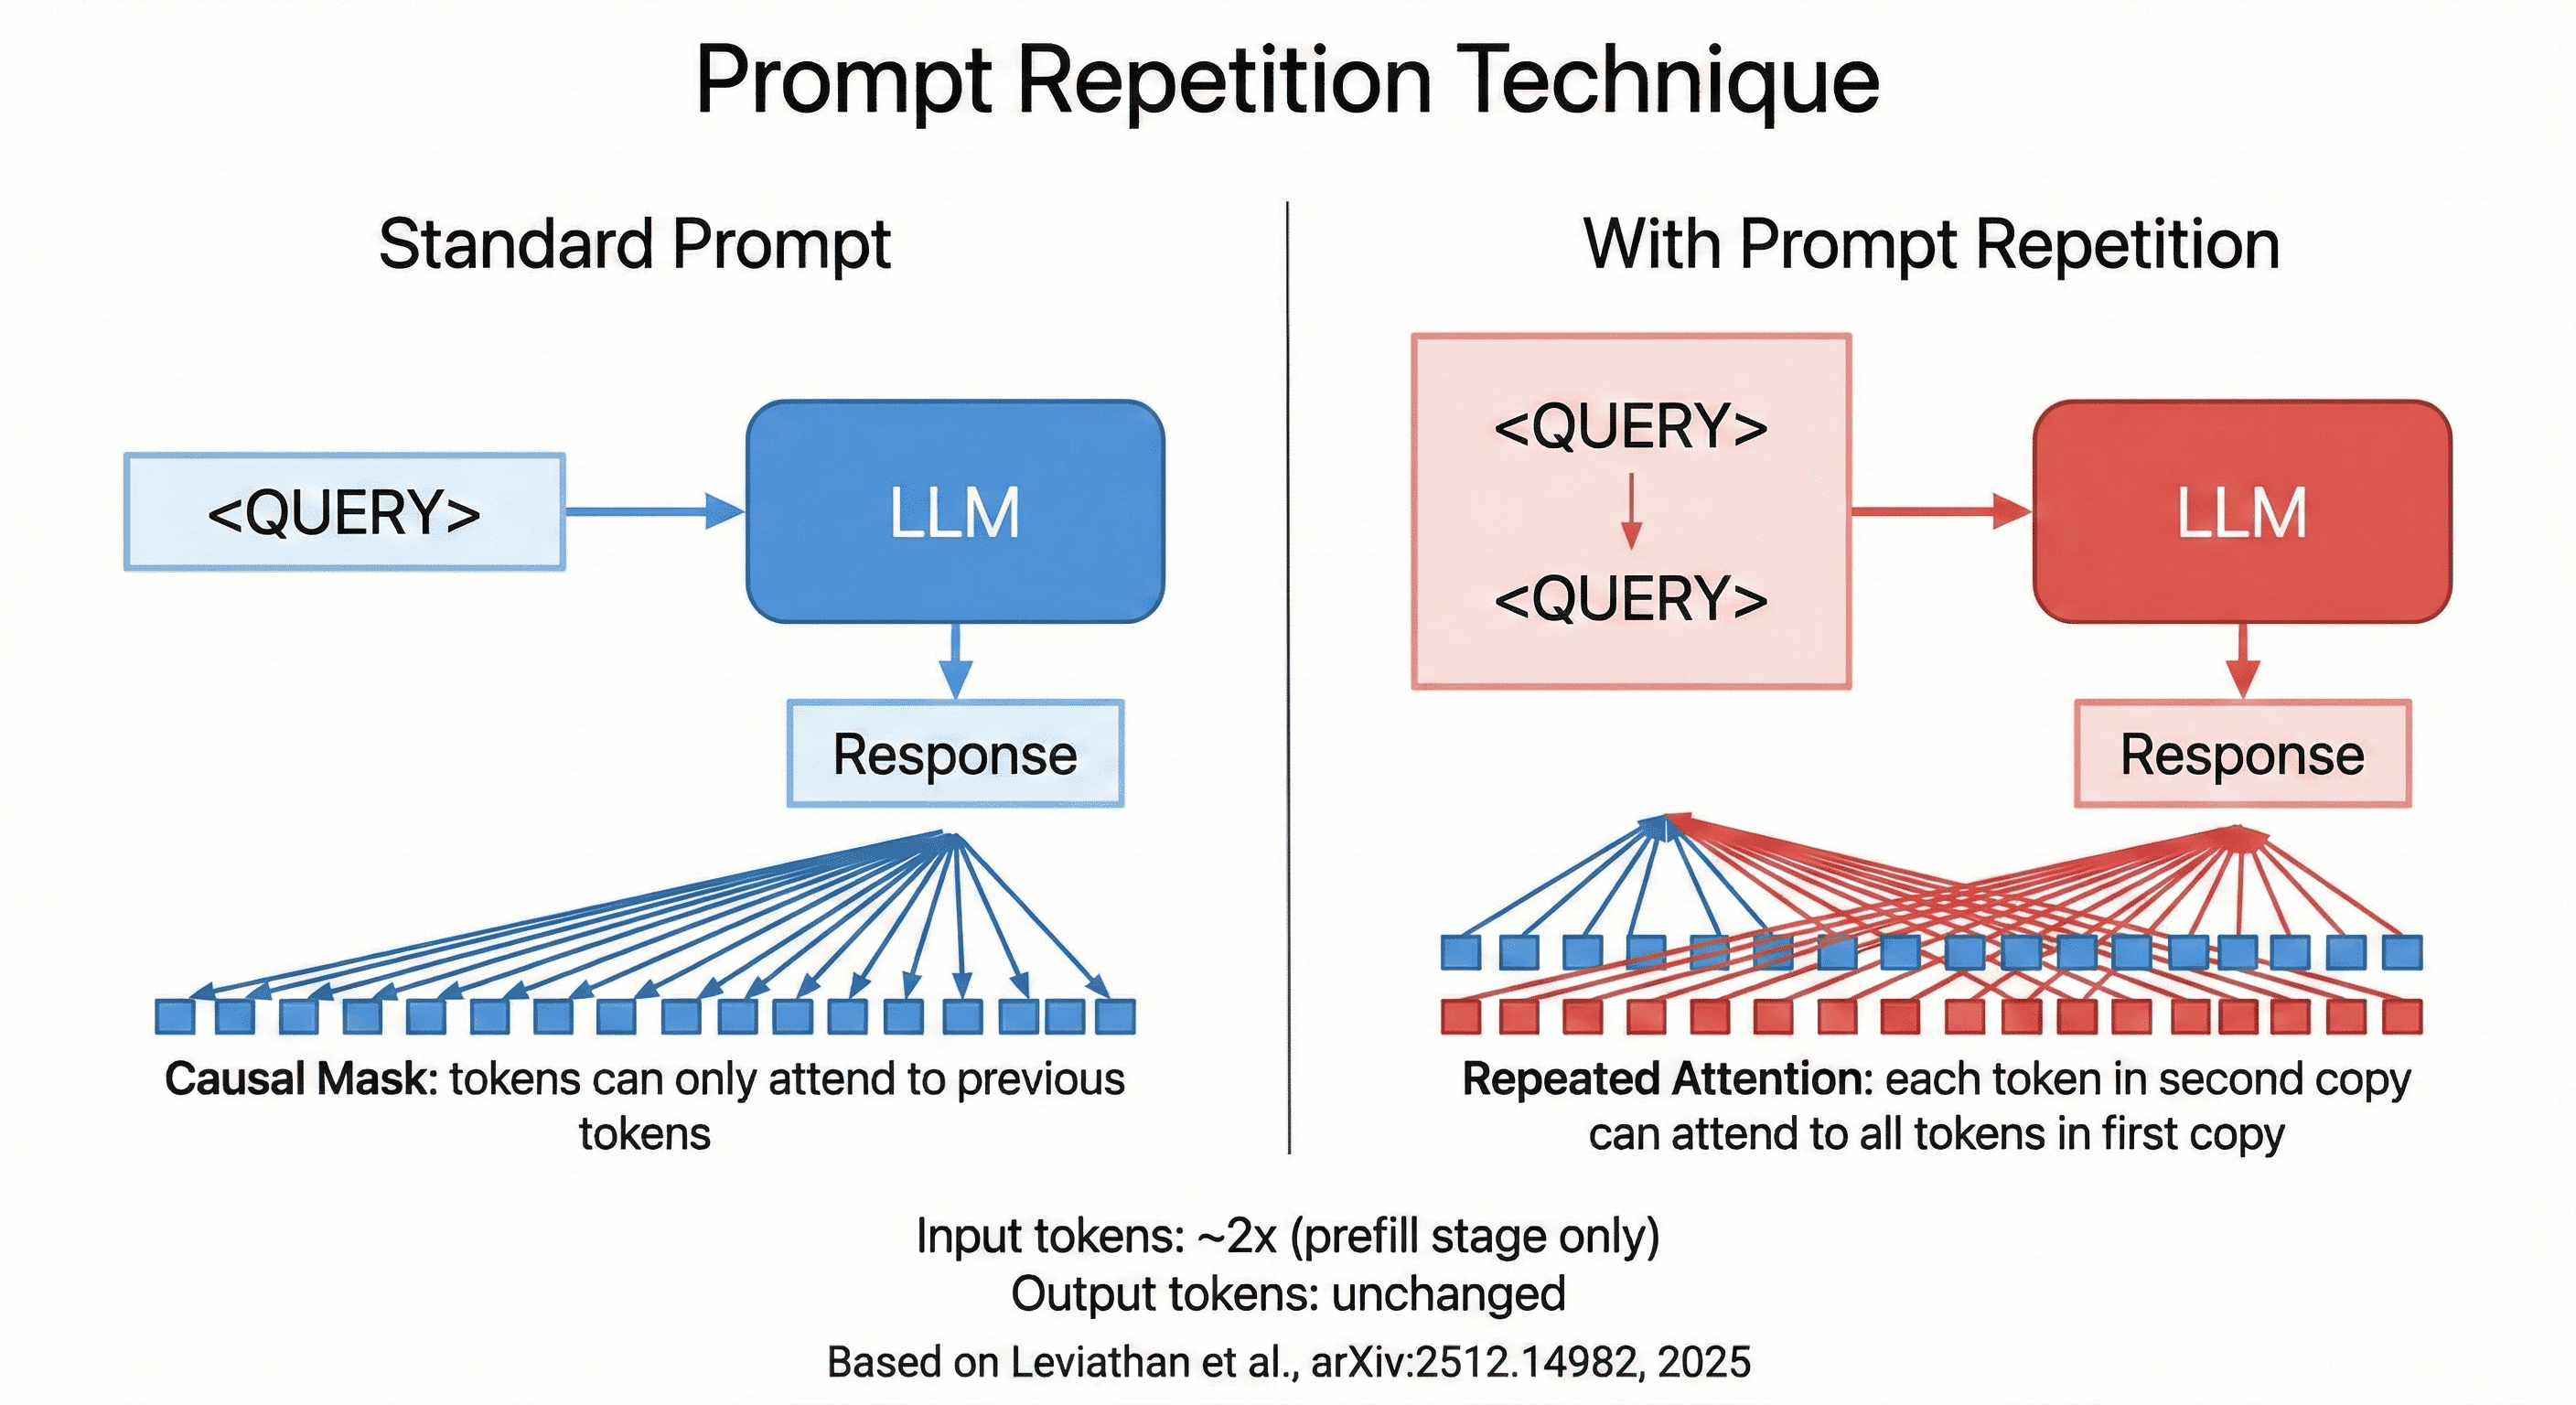
\includegraphics[width=\columnwidth]{figures/PromptRepetition.png}
    \caption{Comparison of attention patterns between standard prompting and prompt repetition. With repetition, tokens in the second copy can attend to all tokens in the first copy.}
    \label{fig:prompt_repetition}
\end{figure}

% -----------------------------------------------------------------------------
\subsection{Implementation Details}
\label{subsec:implementation}

The multi-agent pipeline is implemented using LangGraph, a framework for building stateful, graph-based LLM applications. The workflow is defined as a \texttt{StateGraph} where each agent corresponds to a node, and edges define the execution flow including conditional transitions based on test outcomes.

State management is handled through a \texttt{TypedDict}-based \texttt{GraphState} object that propagates task metadata, planning outputs, generated code, test results, and failure history across nodes. This structured state enables clean separation of concerns and facilitates debugging.

For execution monitoring and debugging, we integrate LangSmith, which provides tracing capabilities for inspecting individual LLM calls, token usage, and execution timelines. This tooling proved essential for diagnosing failure modes and optimizing prompt designs during development.
